% The research methodology as a diagram (TikZ). Build: pdflatex methodology.tex
\documentclass[border=2pt]{standalone}
\usepackage{newtxtext,newtxmath}
\usepackage{tikz}
\usetikzlibrary{positioning,arrows.meta,calc}

\definecolor{ink}{RGB}{33,37,41}
\definecolor{edge}{RGB}{70,90,110}
\definecolor{head}{RGB}{38,84,124}
\definecolor{fillA}{RGB}{232,240,248}
\definecolor{fillB}{RGB}{236,246,238}
\definecolor{fillC}{RGB}{252,243,229}
\definecolor{band}{RGB}{245,245,245}

\tikzset{
  stage/.style={draw=edge, line width=0.6pt, rounded corners=2pt, fill=#1, text width=3.08cm,
                align=left, anchor=north west, inner sep=4pt,
                font=\footnotesize\linespread{0.95}\selectfont, text=ink},
  title/.style={fill=head, text=white, font=\footnotesize\bfseries, minimum width=3.24cm,
                minimum height=0.55cm, inner sep=2pt, anchor=south west, rounded corners=2pt},
  flow/.style={-{Latex[length=2.2mm]}, line width=0.9pt, draw=edge},
}
\newcommand{\pt}{\textbullet\ }
\newcommand{\stagebox}[1]{\parbox[t][5.5cm][t]{\linewidth}{\raggedright\hyphenpenalty=10000 #1}}
\newcommand{\gap}{\par\vspace{3pt}}

\begin{document}
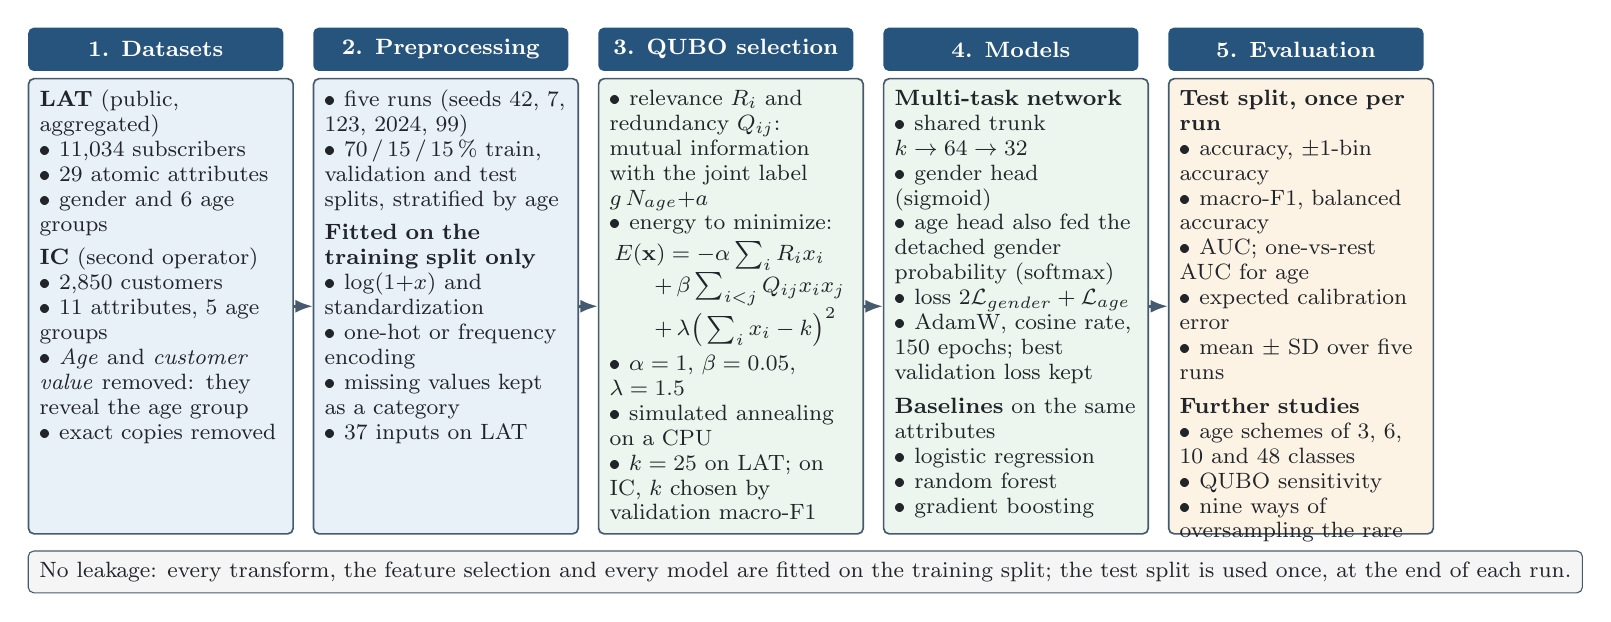
\begin{tikzpicture}
\foreach \i in {1,...,5} { \coordinate (c\i) at ({(\i-1)*3.62},0); }

\node[stage=fillA] (s1) at (c1) {\stagebox{
\textbf{LAT} (public, aggregated)\\
\pt 11{,}034 subscribers\\
\pt 29 atomic attributes\\
\pt gender and 6 age groups\gap
\textbf{IC} (second operator)\\
\pt 2{,}850 customers\\
\pt 11 attributes, 5 age groups\\
\pt \emph{Age} and \emph{customer value} removed: they reveal the age group\\
\pt exact copies removed}};
\node[title] at ($(s1.north west)+(0,0.08)$) {1. Datasets};

\node[stage=fillA] (s2) at (c2) {\stagebox{
\pt five runs (seeds 42, 7, 123, 2024, 99)\\
\pt 70\,/\,15\,/\,15\,\% train, validation and test splits, stratified by age\gap
\textbf{Fitted on the training split only}\\
\pt $\log(1{+}x)$ and standardization\\
\pt one-hot or frequency encoding\\
\pt missing values kept as a category\\
\pt 37 inputs on LAT}};
\node[title] at ($(s2.north west)+(0,0.08)$) {2. Preprocessing};

\node[stage=fillB] (s3) at (c3) {\stagebox{
\pt relevance $R_i$ and redundancy $Q_{ij}$: mutual information with the joint label $g\,N_{age}{+}a$\\
\pt energy to minimize:\\[2pt]
\hspace*{0.2em}$E(\mathbf{x})=-\alpha\textstyle\sum_i R_i x_i$\\
\hspace*{1.9em}$+\,\beta\textstyle\sum_{i<j} Q_{ij}x_ix_j$\\
\hspace*{1.9em}$+\,\lambda\big(\textstyle\sum_i x_i-k\big)^2$\\[2pt]
\pt $\alpha=1$, $\beta=0.05$, $\lambda=1.5$\\
\pt simulated annealing on a CPU\\
\pt $k=25$ on LAT; on IC, $k$ chosen by validation macro-F1}};
\node[title] at ($(s3.north west)+(0,0.08)$) {3. QUBO selection};

\node[stage=fillB] (s4) at (c4) {\stagebox{
\textbf{Multi-task network}\\
\pt shared trunk $k\to64\to32$\\
\pt gender head (sigmoid)\\
\pt age head also fed the detached gender probability (softmax)\\
\pt loss $2\mathcal{L}_{gender}+\mathcal{L}_{age}$\\
\pt AdamW, cosine rate, 150 epochs; best validation loss kept\gap
\textbf{Baselines} on the same attributes\\
\pt logistic regression\\
\pt random forest\\
\pt gradient boosting}};
\node[title] at ($(s4.north west)+(0,0.08)$) {4. Models};

\node[stage=fillC] (s5) at (c5) {\stagebox{
\textbf{Test split, once per run}\\
\pt accuracy, $\pm$1-bin accuracy\\
\pt macro-F1, balanced accuracy\\
\pt AUC; one-vs-rest AUC for age\\
\pt expected calibration error\\
\pt mean $\pm$ SD over five runs\gap
\textbf{Further studies}\\
\pt age schemes of 3, 6, 10 and 48 classes\\
\pt QUBO sensitivity\\
\pt nine ways of oversampling the rare age groups}};
\node[title] at ($(s5.north west)+(0,0.08)$) {5. Evaluation};

\foreach \a/\b in {s1/s2, s2/s3, s3/s4, s4/s5}
  \draw[flow] (\a.east) -- (\b.west);

\path let \p1=(s1.south west), \p2=(s5.south east) in
  node[draw=edge, fill=band, rounded corners=2pt, font=\footnotesize, text=ink, inner sep=4pt,
       minimum width=\x2-\x1, anchor=north west, align=center] at ($(\p1)+(0,-0.2)$)
  {No leakage: every transform, the feature selection and every model are fitted on the training split;
   the test split is used once, at the end of each run.};

\end{tikzpicture}
\end{document}
